\documentclass[border=4pt]{standalone}
\usepackage{amsmath,amssymb}
\usepackage{tikz}
\begin{document}
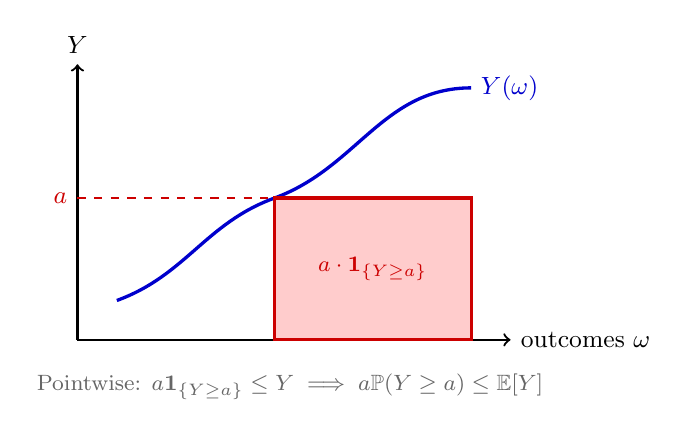
\begin{tikzpicture}[font=\small]
  \draw[->, thick] (0,0) -- (5.5,0) node[right] {outcomes $\omega$};
  \draw[->, thick] (0,0) -- (0,3.5) node[above] {$Y$};

  % Curve Y(omega)
  \draw[very thick, blue!80!black] (0.5, 0.5) to[out=20, in=200] (2.5, 1.8) to[out=20, in=180] (5.0, 3.2);
  \node[right, blue!80!black] at (5.0, 3.2) {$Y(\omega)$};

  % Threshold a
  \draw[thick, dashed, red!80!black] (0, 1.8) node[left] {$a$} -- (5.0, 1.8);

  % Step function a * 1_{Y >= a}
  \draw[very thick, fill=red!20, draw=red!80!black] (2.5, 0) rectangle (5.0, 1.8);
  \node[red!80!black, font=\footnotesize] at (3.75, 0.9) {$a \cdot \mathbf{1}_{\{Y \ge a\}}$};

  \node[font=\footnotesize, text=gray!80!black, align=center] at (2.7, -0.6) 
    {Pointwise: $a \mathbf{1}_{\{Y \ge a\}} \le Y \implies a \mathbb{P}(Y \ge a) \le \mathbb{E}[Y]$};
\end{tikzpicture}
\end{document}